\section{Introduction} \label{sec:intro}
This first chapter gives a general introduction to the wind turbine including both the conventional \textit{fixed-bottom} and floating type. Firstly state of affairs is presented including the motivation for development of floating wind turbine technology. Relevant components and general wind turbine control is furthermore briefly presented followed by a description of the floating wind turbine and the challenges this type faces.


\subsection{State of affairs and motivation} \label{sec:intro_stateofaffairs}
The global average temperature of the earth is rising mainly attributed to the greenhouse effect caused primarily by carbon dioxide (CO2) emissions. The consequences of these temperature changes are aplenty and the more obvious signs of change are already starting to show. Record high temperatures, droughts, storms, floods and other extreme weather conditions and events are becoming more and more frequent. The main contributor of human CO2 emissions is the energy section which represents 76\% of emissions with 42\% resulting from electric energy production \cite{wri2018}. The energy demand on a global scale is still steadily increasing. Due to COVID-19 an unprecedented drop in energy use and CO2 emissions were observed in 2020. But primary energy demand increased again in 2021 by 5.8 \% which was 1.3 \% higher than in 2019 \cite{bp2022}. Fossil fuel still makes up 82 \% of the primary energy use in 2021 \cite{bp2022}. A transition from fossil energies to renewable energy sources is one of the most efficient remedies to lower CO2 emissions and solar and wind energy are widely accepted as some of the best green energy alternatives. Wind and solar reached a 10.2\% share of power generation in 2021 \cite{bp2022}. As of 2021 236 GW of wind power capacity is installed in Europe with 12\% being offshore. 17 GW was installed in 2021 alone with a 19 \% share being offshore wind\cite{Sesto1992}.

\smallskip
Despite the higher levelized cost of energy (LCOE) of offshore wind turbines (WTs) compared to the onshore counterpart the trend towards offshore wind is increasing. There are sensible reasons for this. Offshore wind is on average 20\% higher than onshore. Turbulence is also less due to the lack of obstacles at sea which could potentially extend the expected WT lifetime \cite{Christiansen2013}. Furthermore wind farms at sea do not have the same clearance issues with regards to minimum distance from urban areas and houses. As a result visual and noise annoyances are also decreased. Issues with regards to offshore WTs is the shallow water debt requirement of most types of foundations. Above 50 meters water debt \textit{fixed-bottom} offshore WTs start to become economically infeasible \cite{Lefebvre2012}. Shallow water debt sites will also eventually exhaust and it will become a necessity to install WTs at deeper waters. This is where the floating offshore wind turbine (FOWT) comes into play. Floating turbines have mainly been a research subject in the prototype stage since the first Blue H Technologies FOWT was started up in 2007. It was a prototype installed to gather test data on wind and sea conditions and it was decommissioned at the end of 2008. Despite not having reached full commercial feasibility yet, the FOWT park scale is increasing. Kincardine, the largest floating WT project, was commissioned in 2021 off the coast of Scotland in 60-80 meter waters. The project features 5 Vestas V164-9.5 MW and one V80-2 MW turbine with a combined nominal output of 48 megawatts (MW). Before further exploring FOWTs basic WT functionality is defined.


\subsection{Components and operation of a wind turbine} \label{sec:intro_wtcomponents}
This subsection gives a brief presentation of the relevant WT components and wind turbine control. In \cref{fig:wt_components} a digram of the main components of a WT is seen. Since this report is focused on rotor speed control the most relevant components are the: Blades and rotor, pitch system and generator. Most of the other components also play a role and most will be mentioned more or less throughout the report. 

When the wind, which is also pictured on the diagram, strikes the rotor blades a torque is generated which drives the turbine rotor around. The rotor spins the low-speed shaft which in turn spins the generator through the high-speed shaft. Depending on whether the turbine is operating below or above rated wind speed it will regulate the rotor rotational velocity with either the generator torque or the blade pitch angle. Rated wind speed is a turbine specific wind speed at which rated power output is reached.
Control at below rated wind speed called partial load control (PLC) is done through regulating the generator power or torque with the blade pitch sat at an optimal angle. The generator torque is controlled through the \textit{converter}. Most modern wind turbines are full-scale converter based which means that all the output power of the generator is fed through a converter which is connected to the grid. This gives full control of the power output of the turbine and allows for full control of the generator torque. Control at above rated wind speed called full load control (FLC) is done by regulating the blade pitch angle with the output power or torque held constant.

Furthermore both onshore and fixed-bottom offshore turbines are connected to a firm foundation. Therefore the primary external loads on regular WTs are the wind and gravity.
\begin{figure}[ht]
	\centering
	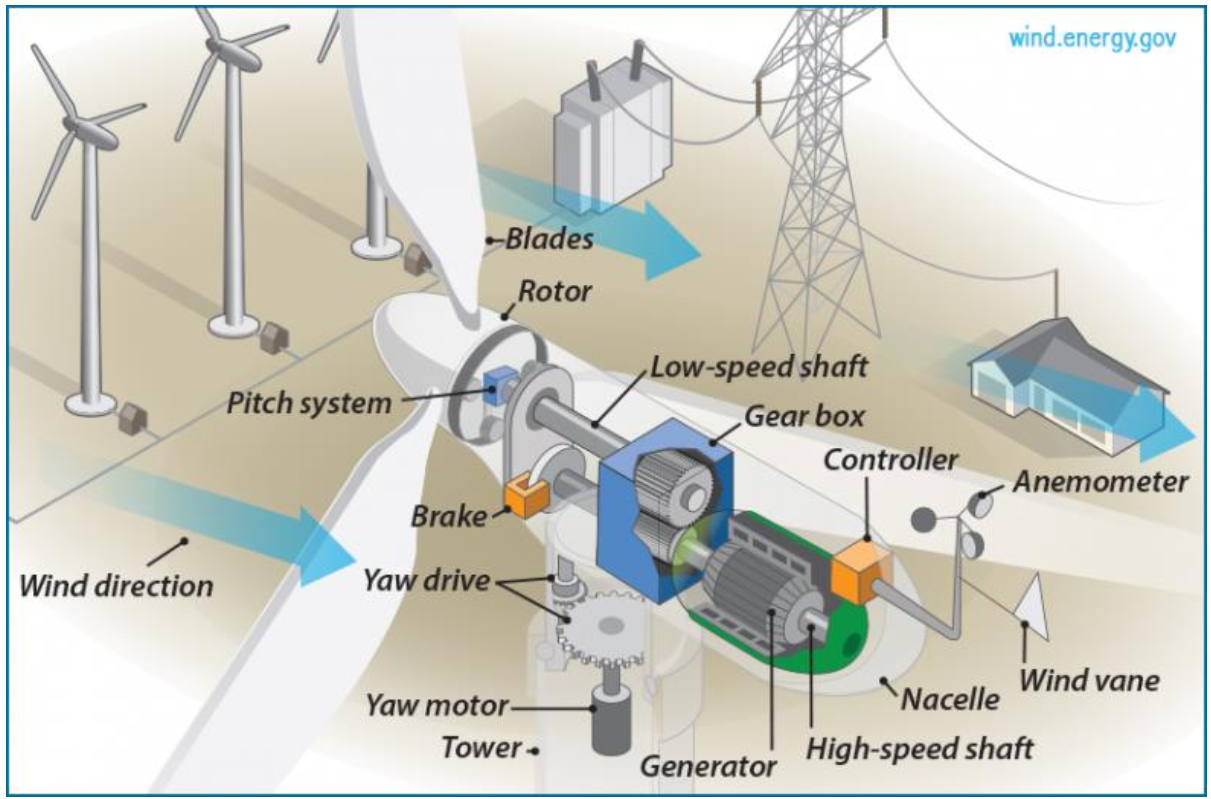
\includegraphics[width=0.7\linewidth]{Graphics/WtComponents.png}
	\caption{Illustration with an overview of the main components which make up a wind turbine}
	\label{fig:wt_components}
\end{figure}


\subsection{The floating offshore wind turbine} \label{sec:intro_theFOWT}
Floating turbines are characterized by having a floating foundation in contrast to the fixed-bottom foundation. Many foundation concepts exist and new ones are continuously proposed but four types are mainly used currently and they are depicted in \cref{fig:floating_concepts}. Each floater type is categorized based on which force is the main driver in keeping the turbine upright in the face of external forces.
\begin{figure}[ht]
	\centering
	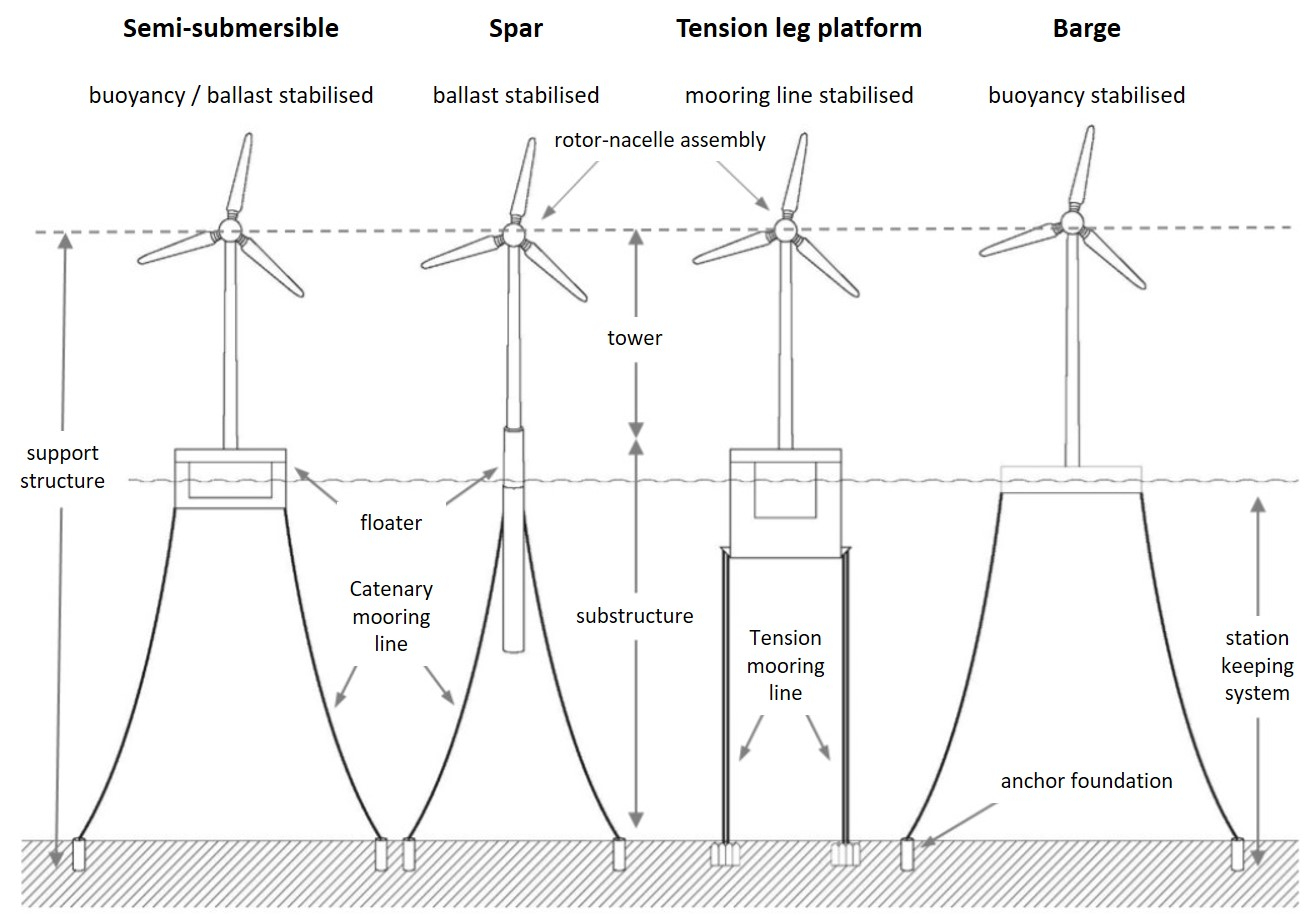
\includegraphics[width=1\linewidth]{Graphics/FloatingFoundationConcepts.jpg}
	\caption{The four main floating foundation concepts: Semi-submersible, Spar boyo, Tension leg platform and the Barge \cite{DNV-GL2018}}
	\label{fig:floating_concepts}
\end{figure}
A characteristic property of floating platforms is static stability which ensures that the overturning moment from the external loads is counteracted. The restoring force can be expressed as a sum of three components: The buoyancy force, the ballast force and the mooring line force where
\begin{itemize}
	\item the \textbf{buoyancy force} is the buoyancy contribution which is dependent on the area of water occupied by the floater
	\item the \textbf{ballast force} is the ballast contribution which is dependent on the distance from the centre of gravity and the centre of buoyancy of the platform.
	\item the \textbf{mooring line} force is the mooring line system contribution.
\end{itemize}
Foundation types in which the buoyancy contribution prevails are called buoyancy-stabilized. Likewise foundations where the ballast and mooring line contributions prevail are ballast and mooring line stabilized respectively. The semi-submersible type is both buoyancy and ballast stabilized. It achieves buoyancy stability by covering a large water-plane area and ballast stability from having three cylinders connected by struts containing ballast weights at the base. Furthermore \textit{heave plates} sit at the bottom of the cylinders yielding increased dampening while adding mass to the system.
Floaters are subjected to additional external loads: Hydrodynamic forces act on the foundation and are comprised of contributions from waves, buoyancy forces and viscous forces. The mooring system will furthermore affect the foundation and differently depending on the type of mooring system.

\smallskip
FOWTs are still in the developmental stage with a higher LCOE than the on- and offshore counterparts. They experiences greater structural strain because of significant rotational and translational motions of the support structure. The illustration in \cref{fig:fowt_coordinates} shows the additional degrees of freedom (DOFs) of FOWTs.
\begin{figure}[ht]
	\centering
	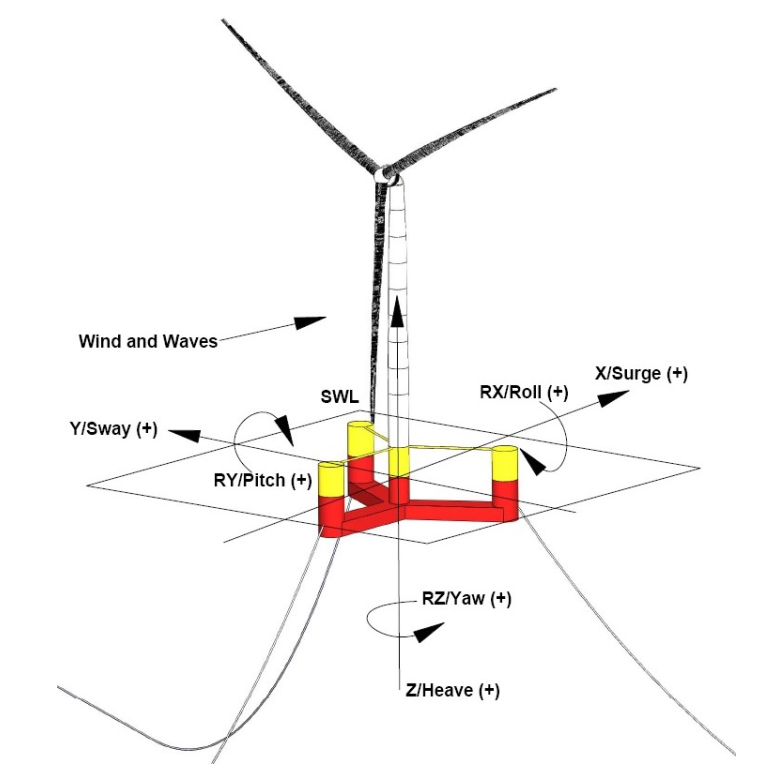
\includegraphics[width=0.55\linewidth]{Graphics/FOWTcoordinates.png}
	\caption{The 6 additional degrees of freedom (DOFs) of a floating offshore wind turbine. The fore-aft motion refers to the \textbf{surge} and \textbf{pitch} motion. Figure is from internal LaC department material made by Thea Vanelli.}
	\label{fig:fowt_coordinates}
\end{figure}
Because of the increased movement, the tower is reinforced to handle the greater loads which increases the LCOE. Therefore it is of great interest to explore methods to dampen the movement of the floating WT structure. One of the large challenges in the FOWT development is handling the negative dampening problem. It is briefly described here and will be examined in greater detail in a later section.

\smallskip
As the wind is flowing through the rotor plane the wind thrusts and pitches the WT backwards. This motion is referred to as the \textit{fore-aft motion}. The backwards thrust changes the relative velocity as seen by the rotor. When the turbine moves backwards the relative wind speed decreases resulting in a decreased torque and thrust. Above nominal wind speeds the WT controller will regulate the rotor speed via the rotor pitch angle which will pitch the blades into the wind to increase the rotational speed. This increases the thrust making the WT move backwards even faster. In the forwards motion the opposite occurs where the pitch is increased to lower the rotor speed which results in an even faster forward motion. The objective of this report is to derive a linear model of a FOWT to use as a control model for reducing the fore-aft motion. 


\subsection{Problem definition} \label{sec:intro_problemdef}
Can a linear model at an operating point capture the fore-aft movement dynamics of a floating wind turbine well enough to be used in a controller to dampen said motion.